\subsection{Architecture logicielle}
\label{archiBP1818}

	Dans cette partie nous allons présenter l'architecture de l'application web développée chez BP1818 et représentée sur la figure \ref{archiFoncBP1818}. Notre équipe est en charge de développer aussi bien la partie frontend que backend de ce projet. Pour cela, différentes technologies ont été choisies peu avant mon arrivée. \\
	
	Notre backend est constitué de plusieurs couches dont une API Rest, nommée Fronting-Business, développée à l'aide du framework Spring en ayant recours à Spring Boot et au langage Java. Cette API regroupe l'ensemble du code source et expose tous les services qui seront consommés par notre frontend. Une seconde couche API Gateway est présente et assure la sécurité ou encore le routage en implémentant la gateway Zuul de la stack Netflix OSS, exactement comme pour le projet chez Neuflize OBC (\ref{microservicesArchi}). Cette gateway est temporairement utilisée durant la phase de développement puis sera remplacée par l'API Gateway d'Axway (\ref{axway}) tout comme chez NOBC. Il existe une troisième API développée pour les besoins du projet à savoir le moteur de scoring MIF. Il permet de calculer le score d'un client de la banque en fonction de ses réponses aux questionnaires MIF et n'a pas été conçu par nos soins mais par une équipe interne de chez Natixis. Nous parlerons plus en détails de ce moteur et de son intérêt dans la partie \ref{moteurScoring}. \\
	
	Dans le but de persister nos données, nous avons recours à une base Couchbase. Cette dernière est une base de données non structurées de type NoSQL dans laquelle tout est persisté sous forme de document au format JSON. Ces documents sont distribués au travers du cluster Couchbase et stockés dans des conteneurs nommés "buckets". Il s'agit de partitions logiques au sein du cluster permettant de grouper différents documents auxquelles on alloue de la mémoire RAM lorsqu'on les crée. Tous les documents se voient attribuer un ID qui est hashé lorsqu'il sont ajoutés en base ensuite de quoi la table de hashage est mise à jour puis stockée dans la mémoire allouée avec les métadonnées du document ce qui permet de garantir des temps d'accès très faibles. Dans notre cas nous avons un cluster contenant trois buckets :
	\begin{itemize}
		\item references : Contient toutes les données de références. Il s'agit des données métiers qui ne sont pas vouées à évoluer (liste de pays, départements en France, pièces justificatives à fournir en cas d'ouverture de compte, etc...)
		\item customers : Contient toutes les données des clients (réponses au questionnaire MIF, données personnelles, contrats souscrits etc...)
		\item customers-test : Bucket créé pour les test unitaires de l'application \\
	\end{itemize}
	
	Durant ce projet, nous avons adopté un paradigme de programmation réactive. Il s'agit d'un type de programmation de plus en plus populaire qui a sans doute représenté, pour moi, la principale difficulté que j'ai rencontré sur ce projet. Il est possible d'avoir recours à des flux d'événements asynchrones (comme des clics souris) que l'on peut observer pour y réagir. Avec la programmation réactive, les flux sont présents partout, et \textbf{tout} peut être un flux, que ce soit les variables, les inputs ou les réponses de requêtes. Ils sont une séquence d'événements ordonnés dans le temps qu'il faut traiter de manière asynchrone en appliquant des fonctions de callback sur les valeurs qu'ils émettent. Cela se rapproche grandement du pattern observer/observable. En effet, afin de pouvoir traiter les événements il faut d'abord écouter le flux (on parle de souscrire à celui-ci) qui est donc l'\textit{observable} puis lui appliquer des fonctions qui sont les \textit{observer}. Les flux sont immutables et peuvent être utilisés de manière chaînée ce qui rend le code très concis et beaucoup plus clair. Concernant les outils, nous avons recours aux bibliothèques \textit{ReactiveX} disponibles dans de nombreux langages (dont java pour notre backend avec RxJava et javascript pour notre frontend avec RxJS). ReactiveX fournit des méthodes et met en place un modèle basé sur les observables pour manipuler les flux de la même manière que les collections à la mode Java 8. La figure \ref{reactivex} illustre un example de programmation réactive.
	
\begin{figure}[h!]
	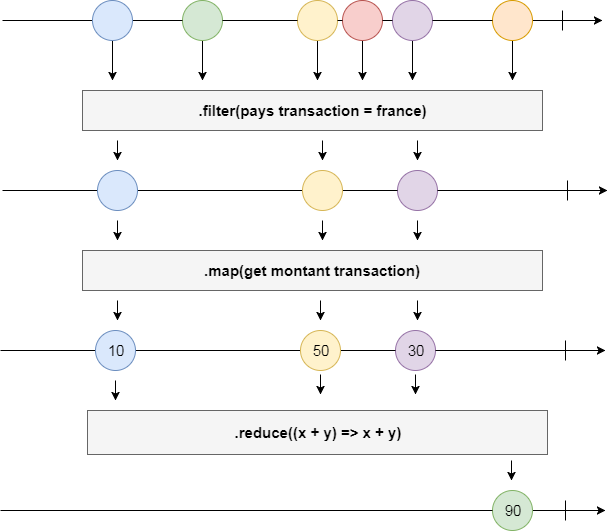
\includegraphics[scale=0.50]{images/travailBP1818/architecture/reactivex.png}
	\centering
	\caption{Example de programmation réactive}
	\label{reactivex}
\end{figure}

	Les rectangles gris sont les méthodes mises à disposition par ReactiveX pour manipuler les flux. Supposons qu'après un appel vers un service on récupère la liste des transactions bancaires effectuées par un client. Ici nous avons recours à ReactiveX et la programmation réactive pour construire un premier flux contenant lesdites transactions (symbolisées par les boules de couleurs). Une première fonction \textit{filter} filtre le flux afin de ne garder que les transactions effectuées en France, puis les émet dans un second flux. Après cela la fonction \textit{map} transforme chaque objet de type transaction en un entier qui est le montant en euros puis émet ces entiers dans un nouveau flux. Enfin, la méthode \textit{reduce} applique une fonction aux deux premiers éléments puis l'applique entre le résultat obtenu et l'élément suivant. Le résultat final contient le montant total des transactions effectuées en France par le client et ne nécessite que quelques lignes de code. De plus, les flux sont asynchrones et pendant qu'ils émettent le reste du code n'est pas bloqué et continu à être exécuté. Si la page web a souscrit au résultat du montant, elle sera notifiée lorsque celui-ci sera calculé et la vue sera mise à jour sans actions de la part du client. \\

	Enfin, du côté frontend, la technologie choisie se prête à merveille à la programmation réactive puisqu'il s'agit d'Angular4. Ce dernier est un framework très puissant utilisant le langage \textit{Typescript}, une surcouche de Javascript et se base sur certains concepts clés tels qu'une architecture orientée composant, le data binding bidirectionnelle (lier une partie de la vue au contrôleur) ou encore l'injection de dépendances.

\begin{figure}[h!]
	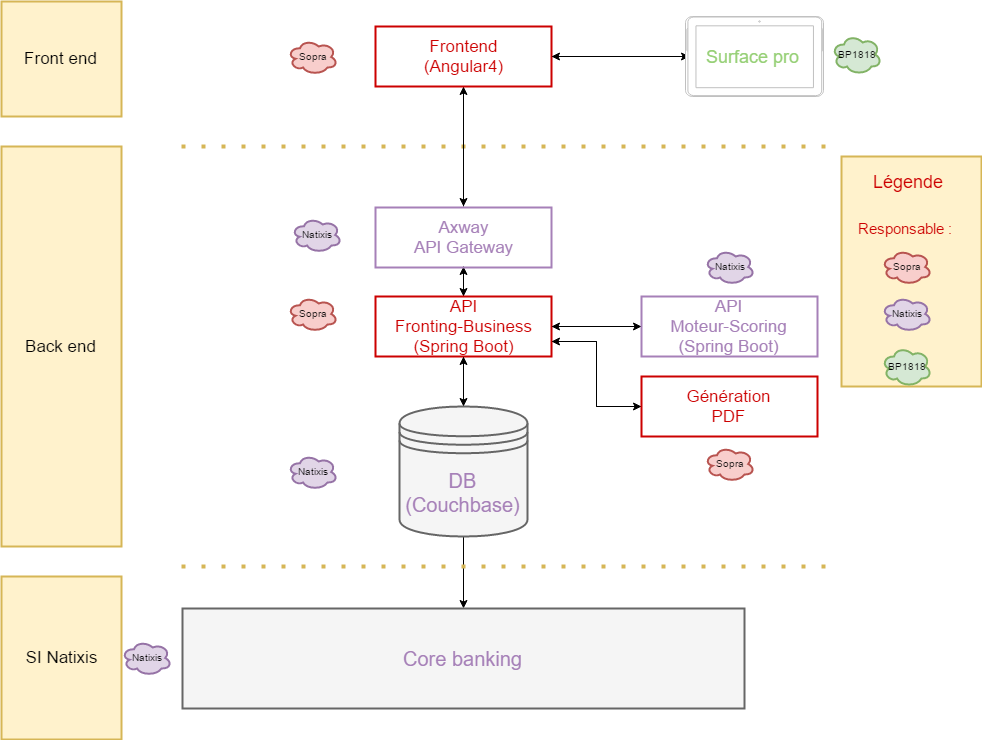
\includegraphics[scale=0.50]{images/travailBP1818/architecture/archiFonc.png}
	\centering
	\caption{Architecture du Fronting Digital}
	\label{archiFoncBP1818}
\end{figure}

\subsection{Conception de l'application}

\subsubsection{Backend}

	Comme nous l'avons dit plus haut, nous avons recours au framework Spring ainsi que Spring Boot dans le but de développer le backend de l'application. L'API fronting-business est construite sur la base d'une Architecture Orientée Services (SOA) qui consiste à traiter l'application comme un fournisseur de services. Dans notre cas, il s'agit de services web RESTful, c'est-à-dire des services suivant les principes REST. Tout comme chez NOBC, l'objectif est de s'affranchir des contraintes portées par les applications monolithiques et mettant en place différents services favorisant la réutilisabilité. En effet, l'API doit être construite de manière à ce que ses services puissent être consommés par divers clients et donc réutilisables afin de s'intégrer le plus simplement possible dans les systèmes d'information des entreprises. \\
	
\begin{figure}[h!]
	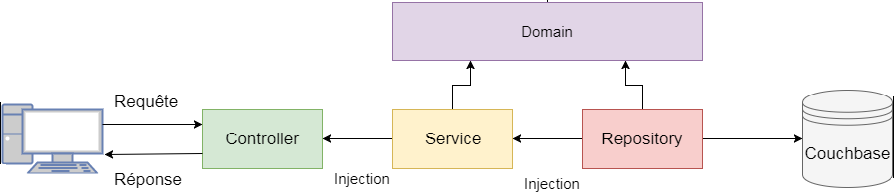
\includegraphics[scale=0.50]{images/travailBP1818/architecture/spring.png}
	\centering
	\caption{Backend Spring Boot}
	\label{spring}
\end{figure}
	
	Ainsi, nous avons mis en place différentes couches, représentées sur le schéma figure \ref{spring}. La couche \textit{controller} réceptionne les requêtes clients et ne manipule pas directement les objects métiers mais passe par des appels de services. C'est dans cette couche que nous définissons l'ensemble de nos endpoints c'est-à-dire les URLs depuis lesquelles le client peut accéder à nos services. Un contrôleur définit les endpoints exposant des services qui possède la même thématique ou qui sont en lien avec la même fonctionnalité c'est pourquoi, généralement, nous avons un contrôleur par user story. \\
	
	La couche \textit{service} contient l'ensemble de nos web services présentant des fonctionnalités unitaires en terme métier. Elle fait abstraction de la compléxité du modèle objet, contient toute la logique des cas d'utilisations permettant d'effectuer les opérations, fournir des données ou encore manipuler les formulaires. Elle implémente la logique métier et gère les appels aux objets de la couche domaine puis valide toutes les règles de gestion métiers. \\
	
	La couche \textit{domain} contient tous nos beans et permet d'implémenter le modèle. \\
	
	La couche \textit{repository} permet de mettre en place la communication avec Couchbase afin de persister les données ou les récupérer. Pour cela, il faut créer un repository. Il s'agit d'une interface contenant toutes les requêtes qu'il est possible d'effectuer sur un document particulier et pouvant être utilisée par injection de dépendance dans un service. Le schéma figure \ref{repository} explicite le fonctionnement de nos repository. \\
	
	Couchbase met à notre disposition une interface, \textit{CouchbasePagingAndSortingRepository<E, ID extends Serializable>}, définissant les requêtes les plus simples et fréquentes comme la sauvegarde d'un document, la recherche ou encore la suppression d'un document par id et gère pour nous les étapes d'ouverture/fermeture de la connexion à la base. Nous n'avons donc rien à implémenter et il suffit de créer un repository héritant de cette interface en spécifiant l'entité que l'on souhaite gérer (E) et le type de la clé (ID). Dans notre cas nous avons une interface, \textit{IdentifiableRepository<E extends IdentifiableDocument>}, héritant de cette dernière qui est notre repository par défaut pour tous les documents. Celle-ci précise lors de son héritage que le type de la clé est \textit{String } et que l'entité est une classe héritant de l'interface \textit{IdentifiableDocument}. Cette interface permet de rajouter et de publier les identifiants d'un document. \\
	
	Ainsi, pour chaque nouveau type de document créé, il suffit de créé un repository héritant à son tour de notre interface générale. Cette procédure permet de grandement économiser du temps et de simplifier le processus de création de nouveau document en favorisant la réutilisabilité.

\begin{figure}[h!]
	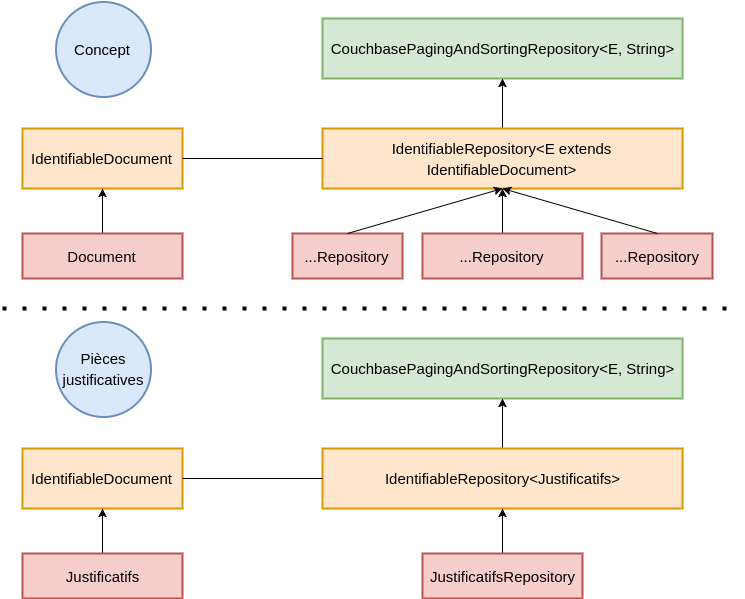
\includegraphics[scale=0.55]{images/travailBP1818/piecesJustif/repository.png}
	\centering
	\caption{Fonctionnement des repositories}
	\label{repository}
\end{figure}

\subsubsection{Frontend}

\hl{TODO : frontend}